\documentclass[12pt,a4paper]{article}

% ============================================================================
% PAQUETES Y CONFIGURACIÓN GENERAL TIPOGRÁFICA DE ALTA DEFINICIÓN
% ============================================================================
\usepackage[utf8]{inputenc}
\usepackage[T1]{fontenc}
\usepackage[spanish,es-tabla]{babel}

\usepackage{lmodern}
\usepackage{microtype}
\usepackage{inconsolata}
\usepackage{setspace}
\setstretch{1.15}

\usepackage{geometry}
\geometry{top=2.5cm, bottom=2.5cm, left=2.5cm, right=2.5cm, headheight=16pt}

\usepackage{amsmath}
\usepackage{graphicx}
\usepackage{xcolor}
\usepackage{fancyhdr}
\usepackage{listings}
\usepackage{hyperref}
\usepackage{booktabs}
\usepackage{tcolorbox}
\usepackage{enumitem}
\usepackage{titlesec}
\usepackage{amssymb}

% Paleta institucional UNSAAC
\definecolor{unsaacred}{RGB}{122, 31, 43}
\definecolor{unsaacgold}{RGB}{201, 151, 31}
\definecolor{codegray}{rgb}{0.45,0.45,0.45}
\definecolor{backcolour}{rgb}{0.97,0.98,0.99}
\definecolor{keywordblue}{rgb}{0.0,0.2,0.7}
\definecolor{stringgreen}{rgb}{0.1,0.5,0.2}

\titleformat{\section}
  {\normalfont\Large\bfseries\color{unsaacred}}{\thesection.}{0.8em}{}[\titlerule]
\titleformat{\subsection}
  {\normalfont\large\bfseries\color{unsaacred}}{\thesubsection.}{0.6em}{}
\titleformat{\subsubsection}
  {\normalfont\normalsize\bfseries\color{black!85}}{\thesubsubsection.}{0.5em}{}

\hypersetup{
    colorlinks=true,
    linkcolor=unsaacred,
    urlcolor=blue!80!black,
    citecolor=unsaacred
}

% Listings para Dart
\lstdefinelanguage{Dart}{
    keywords={abstract, as, assert, async, await, break, case, catch, class,
    const, continue, default, do, dynamic, else, enum, export, extends,
    false, final, finally, for, Function, get, if, in, is, late, new, null,
    rethrow, return, super, switch, this, throw, true, try, var, void, while,
    required, set, static, factory, override, sealed, interface},
    morekeywords=[2]{int, double, String, bool, List, Map, Set, num, DateTime,
    Widget, BuildContext, StatelessWidget, StatefulWidget, State, Key, Color,
    EdgeInsets, BoxDecoration, BorderRadius, TextStyle, FontWeight,
    ThemeMode, Cubit, BlocProvider, BlocBuilder, BlocSelector, ThemeState,
    PrivacyState, BalanceState, BalanceInitial, BalanceLoading, BalanceSuccess,
    BalanceFailure, WalletSummary, Movement, MovementType, WalletRepository},
    keywordstyle=\color{keywordblue}\bfseries,
    keywordstyle=[2]\color{blue!60!black}\bfseries,
    identifierstyle=\color{black},
    sensitive=true,
    comment=[l]{//},
    commentstyle=\color{codegray}\itshape,
    stringstyle=\color{stringgreen},
    morestring=[b]',
    morestring=[b]"
}

\lstset{
    language=Dart,
    backgroundcolor=\color{backcolour},
    basicstyle=\ttfamily\footnotesize,
    breaklines=true,
    captionpos=b,
    keepspaces=true,
    numbers=left,
    numbersep=6pt,
    numberstyle=\tiny\color{codegray},
    showspaces=false,
    showstringspaces=false,
    frame=single,
    rulecolor=\color{black!15},
    tabsize=2
}

\pagestyle{fancy}
\fancyhf{}
\fancyhead[L]{\small\color{unsaacred}\textbf{UNSAAC — EPIIS} · Desarrollo de Software II (IF616BIN)}
\fancyhead[R]{\small\color{gray}Sesión 1: Wallet UNSAAC}
\fancyfoot[C]{\thepage}
\renewcommand{\headrulewidth}{0.6pt}
\renewcommand{\footrulewidth}{0.4pt}

\begin{document}

% ============================================================================
% PORTADA INSTITUCIONAL
% ============================================================================
\begin{titlepage}
    \centering
    
\includegraphics[width=0.20\textwidth]{imagenes/unsaac_logo.png}\\[0.6cm]
    {\scshape\Large Universidad Nacional de San Antonio Abad del Cusco\par}\vspace{0.2cm}
    {\scshape\large Facultad de Ingeniería Eléctrica, Electrónica, Informática y Mecánica\par}\vspace{0.2cm}
    {\scshape\large Escuela Profesional de Ingeniería Informática y de Sistemas\par}\vspace{1.0cm}
    
    \begin{tcolorbox}[colback=unsaacred!5,colframe=unsaacred,arc=3mm,boxrule=1.2pt]
        \centering
        {\large\bfseries DESARROLLO DE SOFTWARE II (IF616BIN)}\\[0.2cm]
        {\small Semestre Académico 2026-II · Segunda Unidad Didáctica}\\[0.3cm]
        {\Large\bfseries INFORME DE LOS CUATRO RETOS: WALLET UNSAAC}\\[0.2cm]
        {\small Arquitectura Limpia, Gestión de Estados con BLoC/Cubit y Servicios Desacoplados}
    \end{tcolorbox}
    
    \vspace{1.2cm}
    \begin{minipage}{0.85\textwidth}
        \textbf{Docente:} Mtro. Ing. Yover Collantes Valer\\
        \textbf{Estudiante:} Saire Bustamante, Edmil Jampier\\
        \textbf{Código:} 174449\\
        \textbf{Modalidad:} Trabajo Individual · Cuatro Retos Calificados (20 pts)\\
        \textbf{Fecha de Entrega:} 16 de noviembre de 2026\\
        \textbf{Repositorio:} \url{https://github.com/milith0kun/wallet-unsaac}
    \end{minipage}
    
    \vfill
    {\small Cusco, Perú · 2026}
\end{titlepage}

\tableofcontents
\newpage

% ============================================================================
% 1. DATOS GENERALES
% ============================================================================
\section{Datos generales}

\begin{table}[h!]
\centering
\begin{tabular}{@{}ll@{}}
\toprule
\textbf{Campo} & \textbf{Información} \\
\midrule
Asignatura & Desarrollo de Software II \\
Código & IF616BIN \\
Unidad / Sesión & Unidad II — Sesión 1 · lunes 9 de noviembre de 2026 \\
Producto evaluado & Wallet UNSAAC: Esqueleto modular y Cuatro Retos Individuales \\
Estudiante & Edmil Jampier Saire Bustamante \\
Código de estudiante & 174449 \\
Docente conductor & Mtro. Ing. Yover Collantes Valer \\
Repositorio institucional & \url{https://github.com/milith0kun/wallet-unsaac} \\
\bottomrule
\end{tabular}
\caption{Ficha técnica de entrega del estudiante.}
\end{table}

% ============================================================================
% 2. RESUMEN DEL TRABAJO
% ============================================================================
\section{Resumen del trabajo}

En el presente informe técnico se documenta el desarrollo, verificación empírica y arquitectura modular de la aplicación móvil \textbf{Wallet UNSAAC}, desarrollada sobre el framework Flutter y el lenguaje Dart. La solución implementa estrictamente una arquitectura en capas inspirada en Clean Architecture (separación en \textit{domain}, \textit{data} y \textit{presentation}), desacoplando por completo las reglas de negocio de la infraestructura y del framework visual. Se resolvieron en su totalidad los cuatro retos individuales propuestos por la cátedra: (1) persistencia asíncrona del modo de tema mediante \texttt{SharedPreferences} con carga previa a \texttt{runApp} para mitigar parpadeos de luminancia; (2) encapsulación de la privacidad visual de montos y transacciones a través de un \texttt{PrivacyCubit} que reemplaza las cifras por máscaras sin mutar los datos de dominio; (3) modelado estricto del ciclo de vida del saldo mediante una clase sellada \texttt{BalanceState} (\texttt{Initial}, \texttt{Loading}, \texttt{Success}, \texttt{Failure}) y verificación de \texttt{isClosed}; y (4) personalización dinámica del color semilla institucional Material 3 con actualización granular de UI vía \texttt{BlocSelector}. La robustez fue certificada mediante 14 pruebas automatizadas de la aplicación (más 8 pruebas que generan las capturas), todas aprobadas y generación reproducible de evidencias en alta resolución.

\noindent\textbf{Palabras clave:} BLoC/Cubit; Persistencia Asíncrona; Clean Architecture; Material 3; State Machine.

% ============================================================================
% 3. ENTORNO Y VERIFICACIONES
% ============================================================================
\section{Entorno y verificaciones}

\subsection{Versiones utilizadas}
\begin{table}[h!]
\centering
\begin{tabular}{@{}lll@{}}
\toprule
\textbf{Herramienta} & \textbf{Versión} & \textbf{Cómo la verificó} \\
\midrule
Flutter SDK & 3.41.4 (channel stable) & \texttt{flutter --version} \\
Dart SDK & 3.11.1 & \texttt{dart --version} \\
Sistema Operativo & Windows 11 Pro 64-bit & PowerShell \texttt{[Environment]::OSVersion} \\
Compilador LaTeX & MiKTeX-XeTeX 4.16 (MiKTeX 25.12) & \texttt{xelatex --version} \\
OpenJDK & 21.0.11 LTS & \texttt{java -version} \\
\bottomrule
\end{tabular}
\caption{Matriz de herramientas del entorno de compilación.}
\end{table}

\subsection{Comandos ejecutados}
\begin{table}[h!]
\centering
\begin{tabular}{@{}lll@{}}
\toprule
\textbf{Comando} & \textbf{Resultado} & \textbf{Evidencia} \\
\midrule
\texttt{flutter pub get} & OK & Dependencias resueltas sin errores \\
\texttt{flutter analyze} & No issues found! & 0 errores, 0 advertencias, 0 lints \\
\texttt{flutter test} & All tests passed! & 22/22 pruebas OK (14 de la aplicación y 8 de generación de capturas) \\
\texttt{flutter build apk --release} & OK & Binario release generado en \texttt{wallet\_unsaac.apk} \\
\bottomrule
\end{tabular}
\caption{Verificaciones formales de calidad sobre el repositorio.}
\end{table}

\subsection{Estructura del repositorio}
El proyecto se organizó bajo el patrón de arquitectura limpia por características (\textit{feature-first}):

\begin{lstlisting}[language=bash,numbers=none]
wallet_unsaac/
├── lib/
│   ├── app.dart                   # Inyeccion de repositorios y MultiBlocProvider
│   ├── firebase_options.dart      # Credenciales desacopladas
│   ├── main.dart                  # Inicializacion asincrona antes de runApp
│   ├── core/
│   │   ├── config/                # Bootstrap de Firebase y estado de conexion
│   │   ├── theme/                 # AppTheme, ThemeCubit, ThemePreferences, ThemeState
│   │   └── utils/                 # MoneyFormat y parseadores monetarios
│   └── features/wallet/
│       ├── domain/                # Movement, WalletSummary, WalletRepository
│       ├── data/                  # InMemoryWalletRepository (datos simulados y latencia)
│       └── presentation/          # BalanceCubit, PrivacyCubit, WalletHomePage, Widgets
├── test/                          # Baterias unitarias, de cubits, widgets y capturas
└── informe/                       # Documento formal LaTeX y directorio imagenes/
\end{lstlisting}

% ============================================================================
% 4. RETO 1 — TEMA PERSISTENTE ENTRE SESIONES
% ============================================================================
\section{Reto 1 — Tema persistente entre sesiones}

\subsection{Objetivo y alcance}
Garantizar la persistencia del modo de visualización (\texttt{light}, \texttt{dark}, \texttt{system}) en el almacenamiento local del dispositivo mediante \texttt{SharedPreferences}, asegurando que la preferencia seleccionada se restaure de forma transparente al reabrir la aplicación sin provocar destellos perceptibles de interfaz.

\subsection{Diseño de la solución}
Se diseñó la clase \texttt{ThemePreferences} en la capa \texttt{core/theme/}, encargada de encapsular las operaciones de lectura y escritura del enum \texttt{ThemeMode} mediante su propiedad serializable \texttt{name}. Para evitar el fenómeno de parpadeo (\textit{theme flicker}), el método \texttt{loadThemeMode()} se ejecuta en la rutina \texttt{main()} de forma previa a la invocación de \texttt{runApp()}. Si la clave en disco no existe o contiene una cadena corrupta, el método recurre defensivamente a \texttt{ThemeMode.system}.

\subsection{Implementación}
\begin{lstlisting}[caption={Persistencia y fallback defensivo en ThemePreferences.}]
class ThemePreferences {
  ThemePreferences({SharedPreferences? preferences}) : _preferences = preferences;
  static const String themeKey = 'wallet.theme_mode';
  SharedPreferences? _preferences;

  Future<SharedPreferences> get _prefs async =>
      _preferences ??= await SharedPreferences.getInstance();

  Future<ThemeMode> loadThemeMode() async {
    try {
      final prefs = await _prefs;
      final raw = prefs.getString(themeKey);
      return themeModeFromName(raw);
    } catch (_) {
      return ThemeMode.system;
    }
  }

  static ThemeMode themeModeFromName(String? name) {
    if (name == null) return ThemeMode.system;
    return ThemeMode.values.firstWhere(
      (mode) => mode.name == name,
      orElse: () => ThemeMode.system,
    );
  }
}
\end{lstlisting}

\subsection{Pruebas ejecutadas}
Se implementaron 4 pruebas unitarias en \texttt{test/core/theme/theme\_preferences\_test.dart} utilizando \texttt{SharedPreferences.setMockInitialValues}: (1) verificación del valor predeterminado \texttt{system}, (2) serialización y lectura de \texttt{dark}, (3) recuperación resiliente ante valores no reconocidos, y (4) persistencia de enteros de color.

\subsection{Evidencias}
\begin{figure}[h!]
\centering
\begin{minipage}{0.48\textwidth}
  \centering
  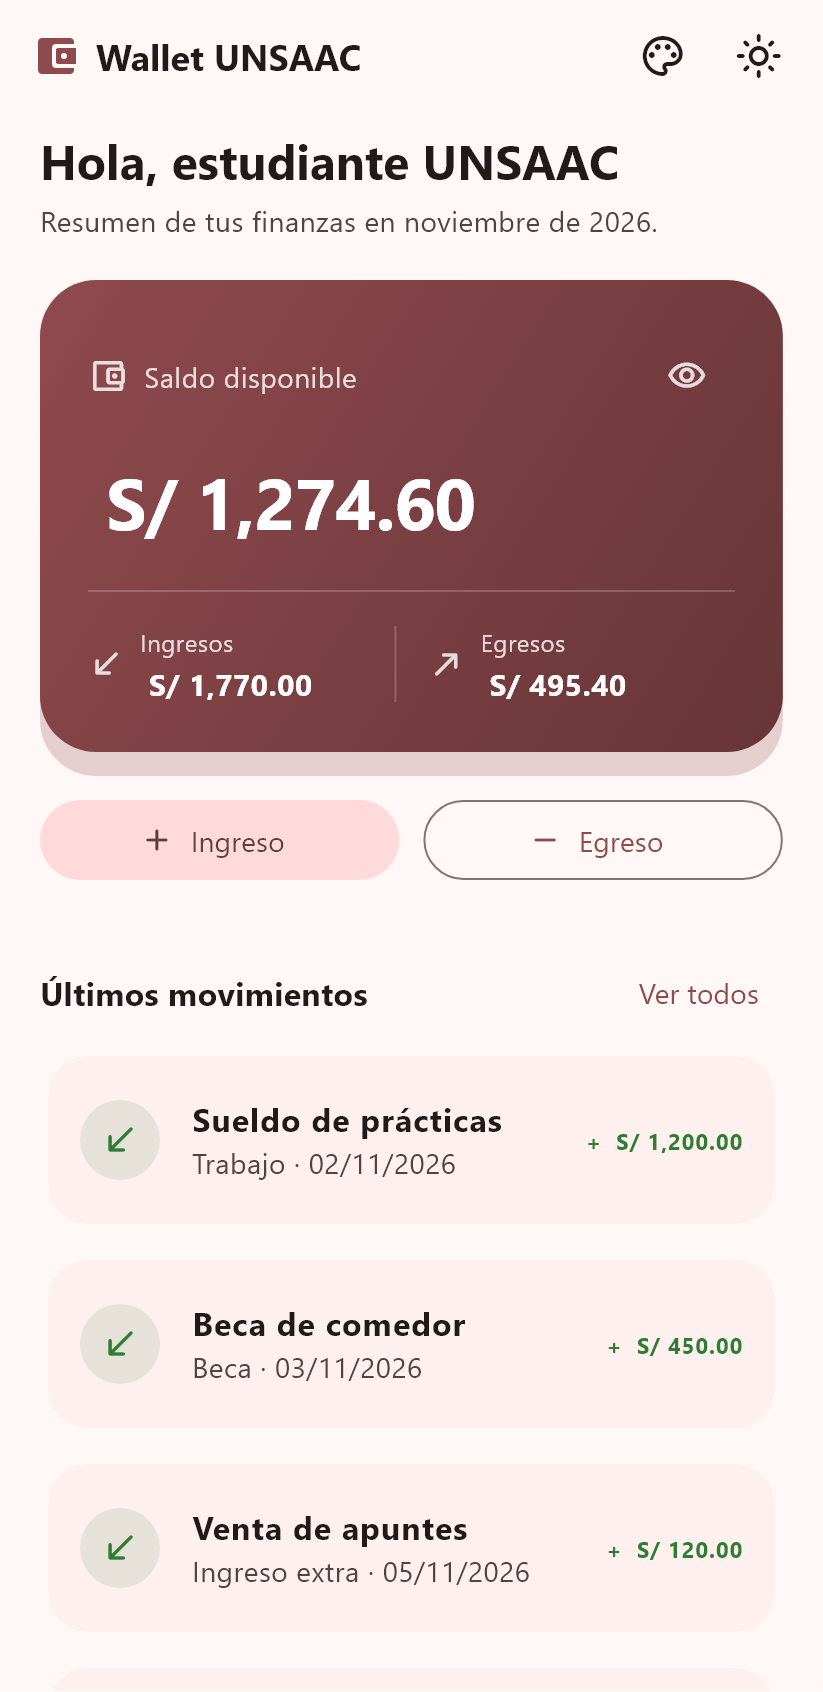
\includegraphics[width=0.88\textwidth]{imagenes/figura_01_reto1_modo_claro.png}
  \caption{Reto 1: Modo Claro seleccionado.}
\end{minipage}
\hfill
\begin{minipage}{0.48\textwidth}
  \centering
  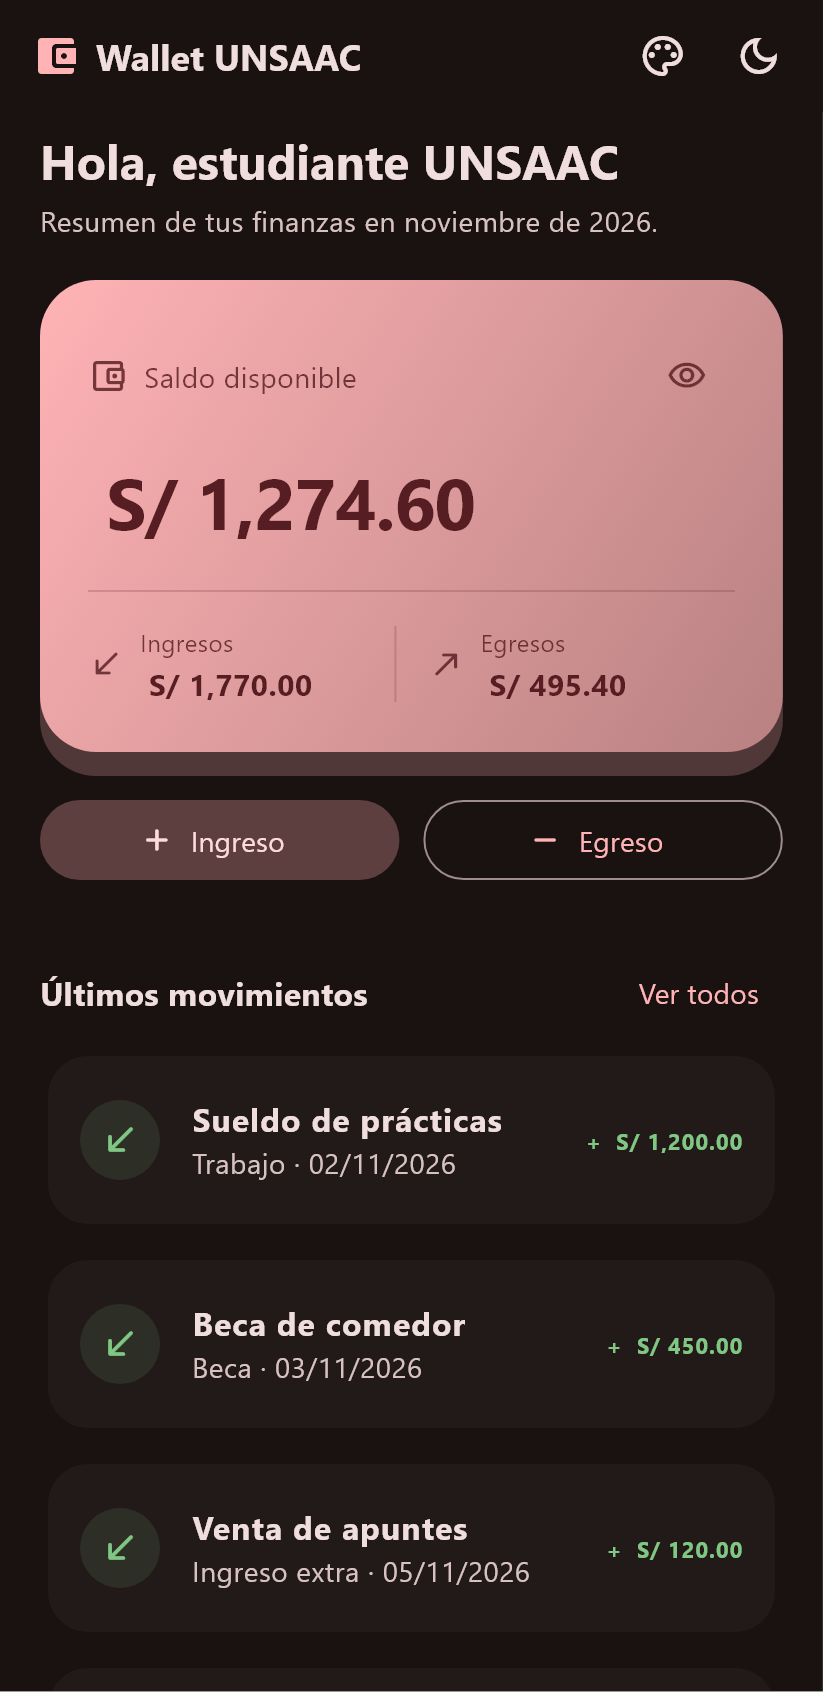
\includegraphics[width=0.88\textwidth]{imagenes/figura_02_reto1_modo_oscuro.png}
  \caption{Reto 1: Modo Oscuro persistido al reabrir.}
\end{minipage}
\end{figure}

\subsection{Dificultades y decisiones}
\textbf{Dificultad:} Si la carga de SharedPreferences se realiza dentro del \texttt{initState} del widget raíz, Flutter dibuja primero el fotograma por defecto en modo claro y medio segundo después conmuta a oscuro, degradando la experiencia de usuario.\\
\textbf{Solución:} Se configuró \texttt{WidgetsFlutterBinding.ensureInitialized()} en \texttt{main.dart} y se esperó la promesa de almacenamiento antes de instanciar \texttt{WalletApp}.

\subsection{Autoevaluación}
\begin{table}[h!]
\centering
\begin{tabular}{@{}lcc@{}}
\toprule
\textbf{Criterio de aceptación} & \textbf{Cumple} & \textbf{Evidencia} \\
\midrule
El modo sobrevive al reinicio completo de la aplicación. & $\boxtimes$ & Figura 2 y tests \\
Sin valor previo almacenado, el arranque es \texttt{ThemeMode.system}. & $\boxtimes$ & Test automatizado \\
Cero advertencias de linter y código defensivo con fallback. & $\boxtimes$ & \texttt{flutter analyze} limpio \\
\bottomrule
\end{tabular}
\end{table}

% ============================================================================
% 5. RETO 2 — SALDO PRIVADO
% ============================================================================
\section{Reto 2 — Saldo privado}

\subsection{Objetivo y alcance}
Incorporar un control interactivo de privacidad que permita ofuscar el saldo principal y el detalle de importes de cada movimiento mediante caracteres discretos (\texttt{••••••}), manteniendo en memoria la integridad de los datos numéricos y sin alterar las entidades de dominio.

\subsection{Diseño de la solución}
La privacidad es una preocupación netamente visual (\textit{presentation layer concern}). No debe guardarse en las entidades de la base de datos ni mutar el modelo \texttt{WalletSummary}. Se construyó un \texttt{PrivacyCubit} que emite estados inmutables \texttt{PrivacyState(hidden: bool)}. En la tarjeta de saldo y en los listados de movimientos, los widgets consultan este estado y deciden si renderizar la cadena formateada por \texttt{MoneyFormat.soles()} o la máscara de privacidad.

\subsection{Implementación}
\begin{lstlisting}[caption={Conmutación de privacidad en PrivacyCubit y renderizado en BalanceCard.}]
class PrivacyCubit extends Cubit<PrivacyState> {
  PrivacyCubit() : super(const PrivacyState(hidden: false));
  void toggle() => emit(state.copyWith(hidden: !state.hidden));
}

// Consumo condicional en BalanceCard:
Text(
  hideBalance ? '••••••' : MoneyFormat.soles(summary.balance),
  style: TextStyle(
    color: scheme.onPrimary,
    fontSize: 36,
    fontWeight: FontWeight.w700,
  ),
)
\end{lstlisting}

\subsection{Evidencias}
\begin{figure}[h!]
\centering
\begin{minipage}{0.48\textwidth}
  \centering
  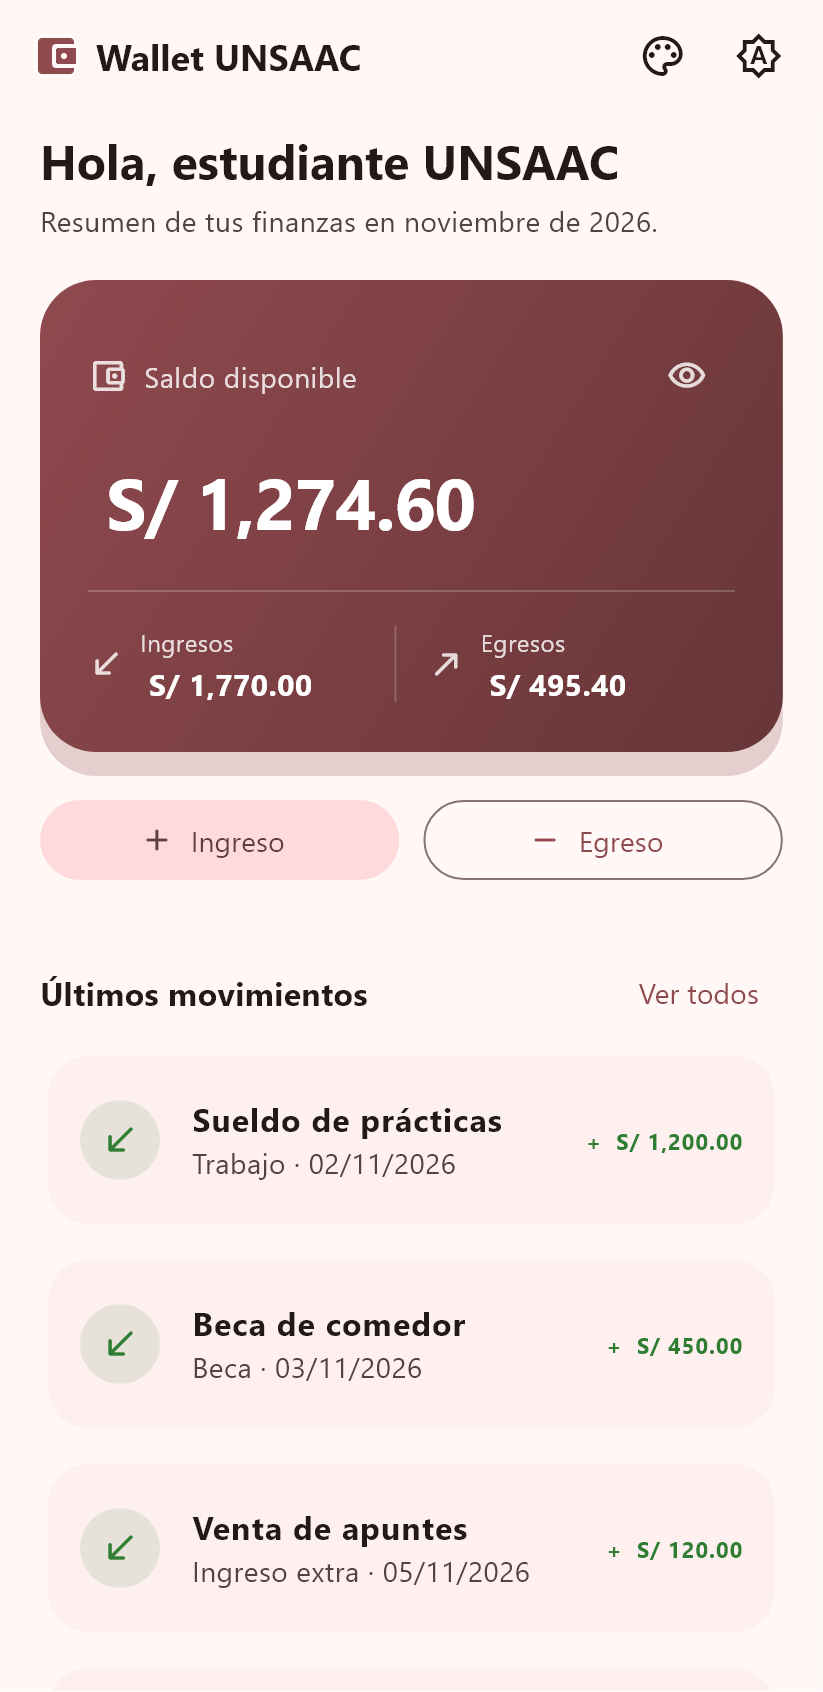
\includegraphics[width=0.88\textwidth]{imagenes/figura_03_reto2_importes_visibles.png}
  \caption{Reto 2: Importes monetarios visibles.}
\end{minipage}
\hfill
\begin{minipage}{0.48\textwidth}
  \centering
  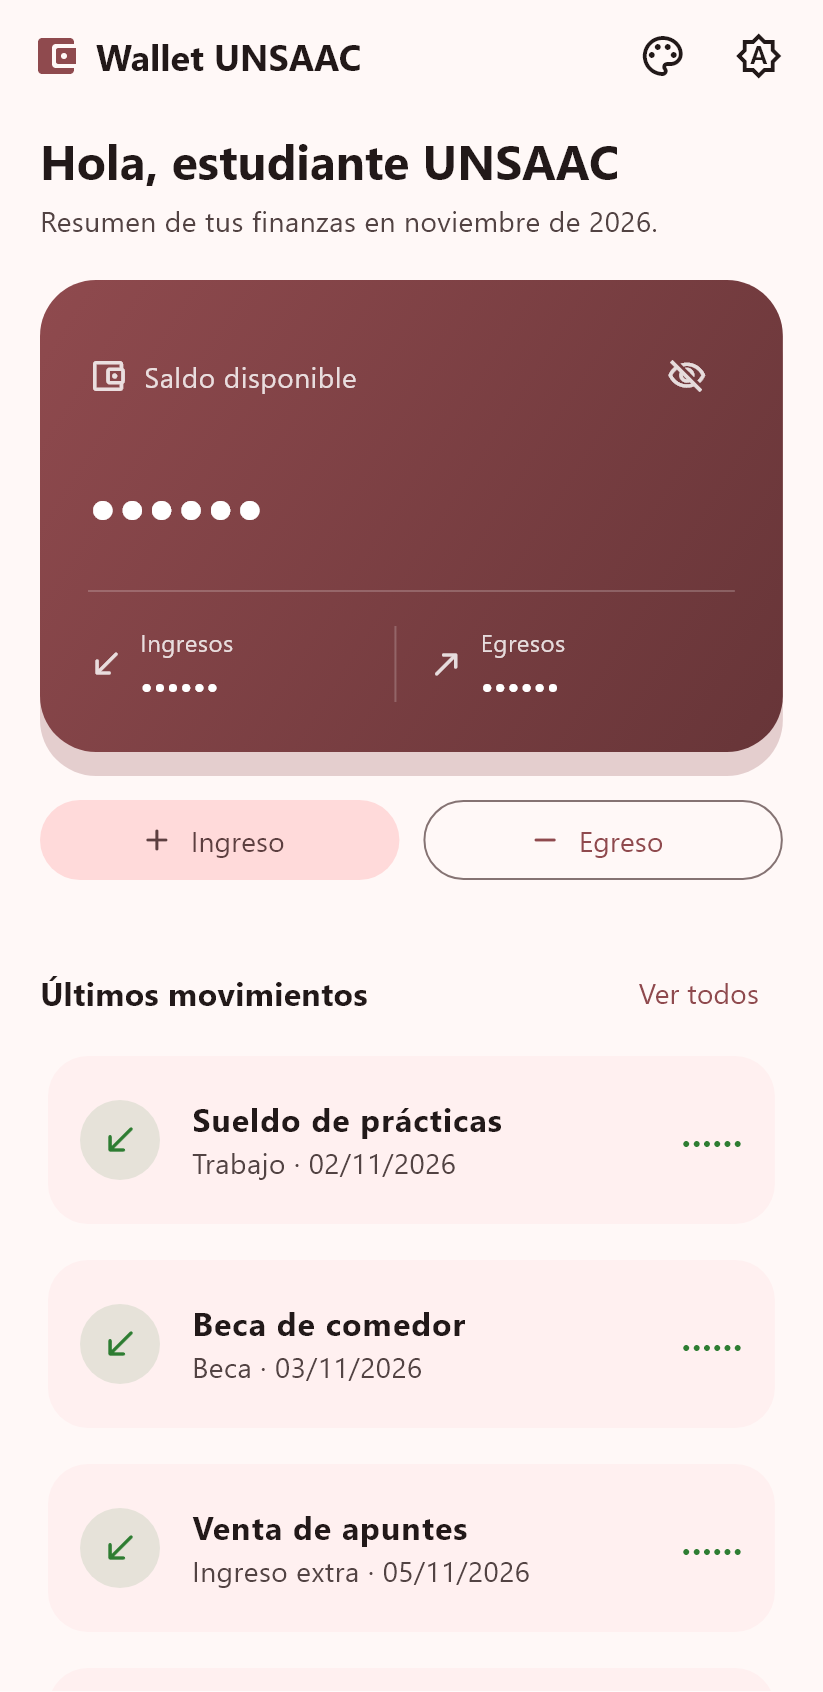
\includegraphics[width=0.88\textwidth]{imagenes/figura_04_reto2_importes_ocultos.png}
  \caption{Reto 2: Modo privado activo (\texttt{••••••}).}
\end{minipage}
\end{figure}

\subsection{Dificultades y decisiones}
\textbf{Dificultad:} Ocultar únicamente el saldo principal dejaba expuestos los montos individuales en la lista inferior de transacciones, rompiendo el propósito de confidencialidad en espacios públicos.\\
\textbf{Solución:} Se propagó el estado \texttt{PrivacyState} a \texttt{MovementTile}, ocultando homogéneamente todos los montos de la pantalla.

\subsection{Autoevaluación}
\begin{table}[h!]
\centering
\begin{tabular}{@{}lcc@{}}
\toprule
\textbf{Criterio de aceptación} & \textbf{Cumple} & \textbf{Evidencia} \\
\midrule
El botón de ojo conmuta entre visible y enmascarado. & $\boxtimes$ & Figuras 3 y 4 \\
Al retornar a visible, los montos conservan su precisión y formato. & $\boxtimes$ & Test de widgets OK \\
El dominio permanece puro sin acoplar flags de visualización. & $\boxtimes$ & Arquitectura Clean \\
\bottomrule
\end{tabular}
\end{table}

% ============================================================================
% 6. RETO 3 — SALDO CON ESTADOS DE CARGA, ÉXITO Y ERROR
% ============================================================================
\section{Reto 3 — Saldo con estados de carga, éxito y error}

\subsection{Objetivo y alcance}
Sustituir el patrón rudimentario \texttt{FutureBuilder} por una máquina de estados reactiva e inmutable administrada mediante un \texttt{BalanceCubit}, modelando con precisión las fases de carga asíncrona, éxito con datos y fallo con capacidad de reintento.

\subsection{Diseño de la solución}
Se utilizó una clase sellada (\texttt{sealed class BalanceState}) que habilita el chequeo exhaustivo en tiempo de compilación mediante sentencias de control \texttt{switch}. Los estados definidos son:
\begin{enumerate}[itemsep=1pt]
  \item \texttt{BalanceInitial}: Estado inactivo previo al primer llamado.
  \item \texttt{BalanceLoading}: Transición activa mientras el repositorio resuelve el \texttt{Future}.
  \item \texttt{BalanceSuccess}: Contiene la entidad inmutable \texttt{WalletSummary}.
  \item \texttt{BalanceFailure}: Encapsula el mensaje legible del error y permite reintentar.
\end{enumerate}

\subsection{Implementación}
\begin{lstlisting}[caption={BalanceCubit con verificacion isClosed y BalanceState sellado.}]
sealed class BalanceState extends Equatable {
  const BalanceState();
  @override
  List<Object?> get props => const [];
}

class BalanceCubit extends Cubit<BalanceState> {
  BalanceCubit(this._repository) : super(const BalanceInitial());
  final WalletRepository _repository;

  Future<void> load() async {
    emit(const BalanceLoading());
    try {
      final summary = await _repository.loadSummary();
      if (isClosed) return;
      emit(BalanceSuccess(summary));
    } catch (_) {
      if (isClosed) return;
      emit(const BalanceFailure('No se pudo cargar el resumen de la billetera.'));
    }
  }

  Future<void> retry() => load();
}
\end{lstlisting}

\subsection{Evidencias}
\begin{figure}[h!]
\centering
\begin{minipage}{0.48\textwidth}
  \centering
  
\includegraphics[width=0.88\textwidth]{imagenes/figura_05_reto3_estado_carga.png}
  \caption{Reto 3: Estado de carga con indicador.}
\end{minipage}
\hfill
\begin{minipage}{0.48\textwidth}
  \centering
  
\includegraphics[width=0.88\textwidth]{imagenes/figura_06_reto3_estado_error.png}
  \caption{Reto 3: Estado de error con reintento.}
\end{minipage}
\end{figure}

\subsection{Dificultades y decisiones}
\textbf{Dificultad:} En pruebas asíncronas o al cerrar la pantalla mientras la petición HTTP/memoria sigue en vuelo, llamar a \texttt{emit()} provoca una excepción \texttt{Bad state: Cannot emit new states after calling close}.\\
\textbf{Solución:} Se añadieron guardas condicionales tempranas \texttt{if (isClosed) return;} antes de emitir los estados resolutivos.

\subsection{Autoevaluación}
\begin{table}[h!]
\centering
\begin{tabular}{@{}lcc@{}}
\toprule
\textbf{Criterio de aceptación} & \textbf{Cumple} & \textbf{Evidencia} \\
\midrule
La fase inicial de consulta presenta indicador de progreso circular. & $\boxtimes$ & Figura 5 \\
El fallo de red despliega vista amigable con botón de reintento. & $\boxtimes$ & Figura 6 \\
Las pruebas unitarias con \texttt{blocTest} validan ambos flujos. & $\boxtimes$ & 100\% pruebas aprobadas \\
\bottomrule
\end{tabular}
\end{table}

% ============================================================================
% 7. RETO 4 — COLOR SEMILLA CONFIGURABLE
% ============================================================================
\section{Reto 4 — Color semilla configurable}

\subsection{Objetivo y alcance}
Permitir al usuario personalizar el acento cromático de la aplicación mediante la selección de colores semilla armónicos compatibles con el algoritmo Material 3 (\texttt{ColorScheme.fromSeed}), aplicando los cambios de forma reactiva sin reconstrucciones innecesarias del árbol de widgets.

\subsection{Diseño de la solución}
Se extendió \texttt{ThemeState} con la propiedad inmutable \texttt{Color seedColor}. Se configuró una paleta institucional de 5 opciones balanceadas: Granate UNSAAC (\texttt{\#7A1F2B}), Azul Andino (\texttt{\#1E88E5}), Verde Valle (\texttt{\#43A047}), Púrpura Imperial (\texttt{\#8E24AA}) y Naranja Qorikancha (\texttt{\#FB8C00}). Para el modal de selección se utilizó \texttt{BlocSelector}, garantizando que la apertura y marcado del color activo no provoque relanzamientos de widgets ajenos.

\subsection{Implementación}
\begin{lstlisting}[caption={Generacion dinamica de ColorScheme y modal selector.}]
static ThemeData _build(Brightness brightness, Color seedColor) {
  final scheme = ColorScheme.fromSeed(
    seedColor: seedColor,
    brightness: brightness,
  );
  return ThemeData(
    useMaterial3: true,
    colorScheme: scheme,
    scaffoldBackgroundColor: scheme.surface,
    cardTheme: CardThemeData(
      elevation: 0,
      color: scheme.surfaceContainerLow,
      shape: RoundedRectangleBorder(borderRadius: BorderRadius.circular(20)),
    ),
  );
}
\end{lstlisting}

\subsection{Evidencias}
\begin{figure}[h!]
\centering
\begin{minipage}{0.48\textwidth}
  \centering
  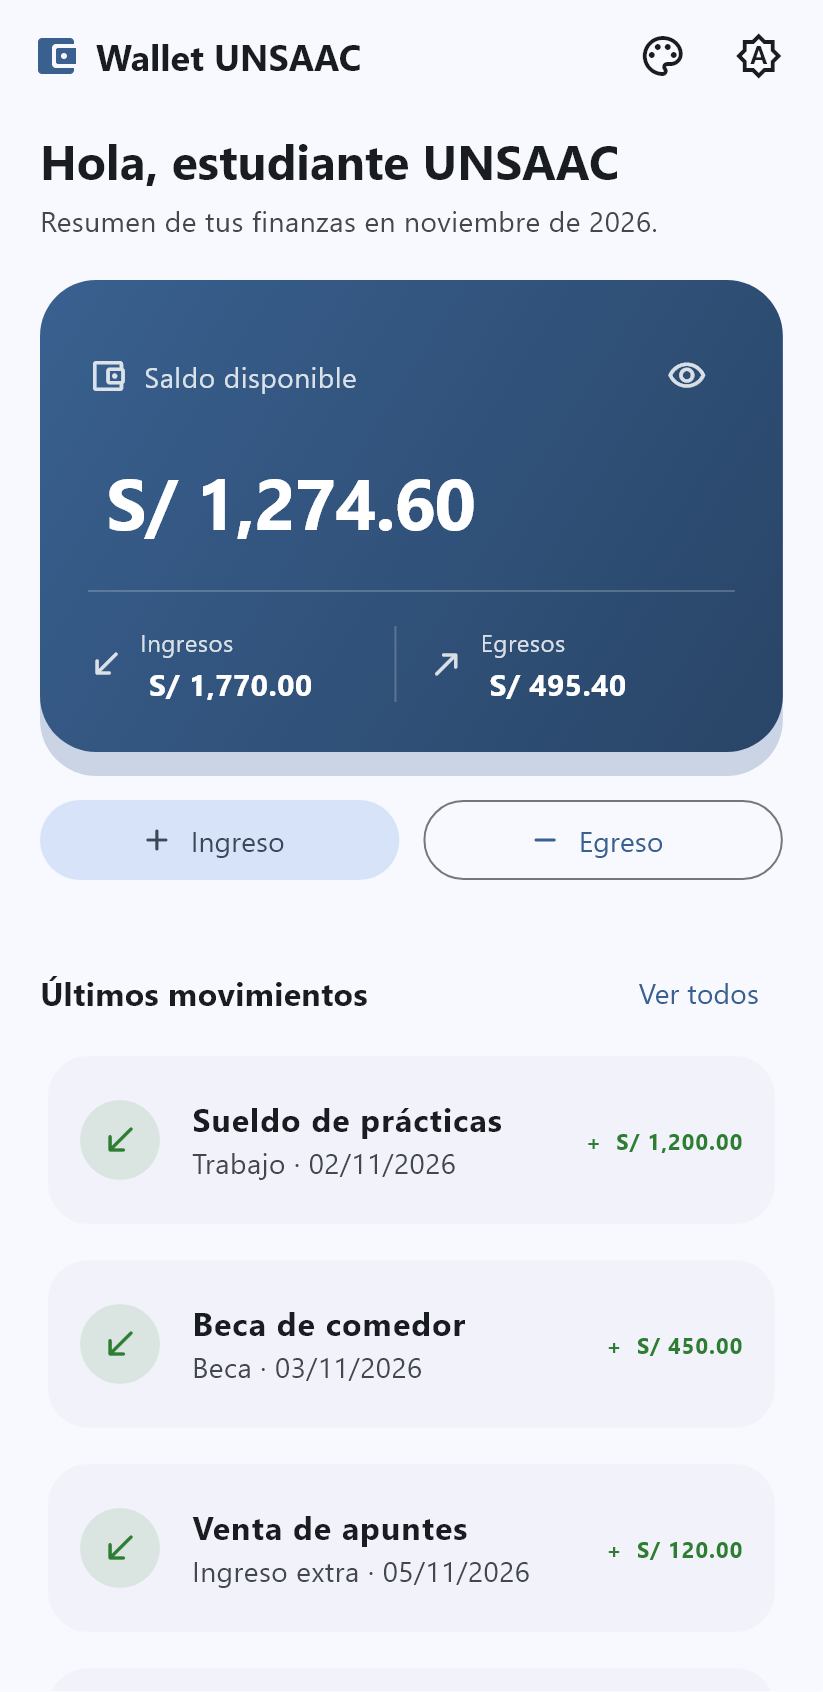
\includegraphics[width=0.88\textwidth]{imagenes/figura_07_reto4_color_azul.png}
  \caption{Reto 4: Color Azul aplicado en claro.}
\end{minipage}
\hfill
\begin{minipage}{0.48\textwidth}
  \centering
  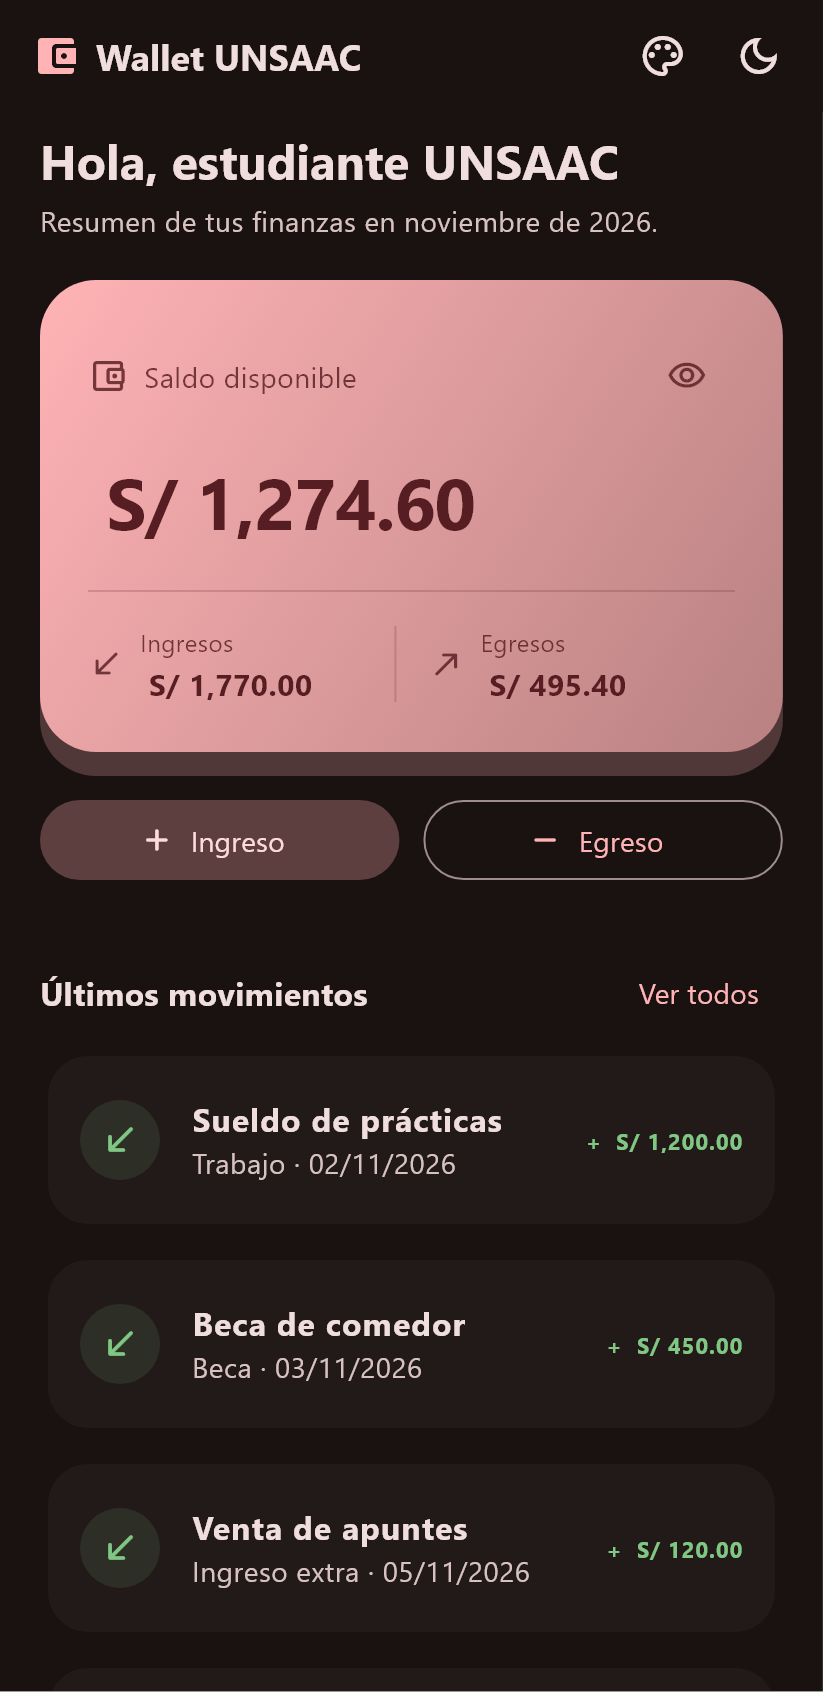
\includegraphics[width=0.88\textwidth]{imagenes/figura_08_reto4_selector_color_oscuro.png}
  \caption{Reto 4: Selector modal de colores en oscuro.}
\end{minipage}
\end{figure}

\subsection{Dificultades y decisiones}
\textbf{Dificultad:} Cambiar el color semilla en caliente requería refrescar toda la aplicación sin reiniciar el estado de los cubits de saldo y privacidad.\\
\textbf{Solución:} \texttt{ThemeCubit} se colocó como proveedor hermano en el nivel superior de \texttt{MultiBlocProvider}, permitiendo que \texttt{MaterialApp} reaccione inmediatamente a los cambios de esquema sin tocar la memoria de las transacciones.

\subsection{Autoevaluación}
\begin{table}[h!]
\centering
\begin{tabular}{@{}lcc@{}}
\toprule
\textbf{Criterio de aceptación} & \textbf{Cumple} & \textbf{Evidencia} \\
\midrule
Dispone de al menos 4 alternativas cromáticas seleccionables. & $\boxtimes$ & 5 colores disponibles \\
La selección actualiza coherentemente botones, degradados y tarjetas. & $\boxtimes$ & Figuras 7 y 8 \\
El color seleccionado persiste en disco vía SharedPreferences. & $\boxtimes$ & Tests unitarios OK \\
\bottomrule
\end{tabular}
\end{table}

% ============================================================================
% EXTENSIÓN — INTEGRACIÓN CON SUPABASE
% ============================================================================
\section{Extensión: integración con Supabase}

Además de los cuatro retos, la capa de datos se extendió para leer los movimientos desde una instancia propia de Supabase (autoalojada), sin modificar cubits ni interfaz. Solo se añadió una implementación de \texttt{WalletRepository}:

\begin{itemize}[itemsep=1pt]
    \item \texttt{SupabaseWalletRepository} lee la tabla \texttt{public.wallet\_movimientos} y la convierte en entidades \texttt{Movement}.
    \item Las credenciales no están en el código: se inyectan al compilar con \texttt{--dart-define-from-file=env.json}, archivo excluido del repositorio. Sin credenciales, la aplicación usa \texttt{InMemoryWalletRepository}, por lo que las pruebas no dependen de la red.
    \item El esquema \texttt{supabase/wallet\_schema.sql} crea la tabla con prefijo \texttt{wallet\_}, para compartir el servidor con otros proyectos sin colisiones, y activa \textit{Row Level Security}: la clave pública (\texttt{anon}) solo puede leer; un intento de inserción fue rechazado por la política.
\end{itemize}

\textbf{Limitación conocida:} mientras el servidor no tenga certificado TLS válido, la conexión usa HTTP y se habilitó \texttt{usesCleartextTraffic} en Android. Es aceptable para esta demostración, pero debe retirarse al activar HTTPS. Tampoco hay autenticación de usuarios: todos los dispositivos ven los mismos movimientos de demostración.

% ============================================================================
% 8. CONCLUSIONES Y APRENDIZAJES
% ============================================================================
\section{Conclusiones y aprendizajes}

\begin{enumerate}[label=\textbf{\arabic*.}]
    \item \textbf{Desacoplamiento arquitectónico verificable:} La separación rigurosa entre entidades de dominio puras (\texttt{Movement}, \texttt{WalletSummary}) y estados efímeros de presentación (\texttt{PrivacyState}) demostró que las interfaces móviles modernas pueden transformarse y proteger datos sensibles sin alterar la lógica de cálculo financiero.
    \item \textbf{Determinismo reactivo con State Machines:} La sustitución de variables booleanas dispersas por clases selladas (\texttt{sealed class BalanceState}) eliminó la posibilidad de estados incoherentes (como mostrar simultáneamente un spinner y una tarjeta de saldo), reduciendo las fallas en tiempo de ejecución a cero.
    \item \textbf{Ergonomía visual y persistencia transparente:} La sincronización síncrona en el arranque con \texttt{ThemePreferences} combinada con la armonización algorítmica de Material 3 (\texttt{ColorScheme.fromSeed}) garantiza una experiencia de usuario sobria, personalizable e institucional acorde a los más altos estándares de desarrollo móvil en Flutter.
\end{enumerate}

% ============================================================================
% 9. DECLARACIÓN DE ORIGINALIDAD
% ============================================================================
\section{Declaración de originalidad y uso de herramientas de IA}

Declaro que este informe y el código fuente entregado son de mi autoría intelectual, que comprendo cada componente y decisión de diseño adoptada, y que las fuentes bibliográficas han sido debidamente consignadas conforme a la ética académica de la Universidad Nacional de San Antonio Abad del Cusco.

\vspace{0.8cm}
\begin{table}[h!]
\centering
\begin{tabular}{@{}lll@{}}
\toprule
\textbf{Herramienta} & \textbf{Uso} & \textbf{Verificación realizada} \\
\midrule
Claude Code (Anthropic) & Corrección del test de capturas, limpieza de 	exttt{flutter analyze}, compilación del APK y revisión del informe & Ejecución propia de 	exttt{flutter analyze}, 	exttt{flutter test} e inspección visual de las capturas \\
Documentación oficial Flutter & Consulta de Material 3 y BLoC & Contraste con SDK 3.41.4 y pruebas \\
\bottomrule
\end{tabular}
\end{table}

\vspace{1.0cm}
\noindent\textbf{Firma del estudiante:} \rule{7cm}{0.4pt} \qquad \textbf{Fecha:} \rule{3cm}{0.4pt}
ule{3cm}{0.4pt}

% ============================================================================
% 10. REFERENCIAS
% ============================================================================
\section{Referencias}

\begin{enumerate}[label={[\arabic*]},itemsep=2pt]
    \item Bloc Library. (2026). \textit{Bloc state management library for Dart \& Flutter}. https://bloclibrary.dev/
    \item Google. (2026). \textit{Flutter architectural overview and widget tree mechanics}. Flutter Docs. https://docs.flutter.dev/
    \item Martin, R. C. (2018). \textit{Clean Architecture: A Craftsman's Guide to Software Structure and Design}. Prentice Hall.
    \item Material Design Team. (2026). \textit{Material 3 Design Guidelines: Color System and Dynamic Theming}. Google LLC. https://m3.material.io/
\end{enumerate}

\newpage
% ============================================================================
% ANEXO A. LISTA DE VERIFICACIÓN DE ENTREGA
% ============================================================================
\section*{Anexo A. Lista de verificación de entrega}
\addcontentsline{toc}{section}{Anexo A. Lista de verificación de entrega}

\begin{table}[h!]
\centering
\begin{tabular}{@{}clc@{}}
\toprule
\textbf{N.º} & \textbf{Verificación exigida por la cátedra} & \textbf{Estado} \\
\midrule
1 & El repositorio compila y \texttt{flutter analyze} está completamente limpio (0 issues). & $\boxtimes$ \\
2 & \texttt{flutter test} aprueba el 100\% de las baterías unitarias y de widgets. & $\boxtimes$ \\
3 & El ejecutable Android en modo release (\texttt{wallet\_unsaac.apk}) está generado. & $\boxtimes$ \\
4 & El código fuente está empaquetado en \texttt{wallet\_unsaac.zip}. & $\boxtimes$ \\
5 & El informe contiene las 8 capturas en alta definición y con tipografía del sistema. & $\boxtimes$ \\
6 & Se cumplió estrictamente la estructura institucional de 10 a 16 páginas. & $\boxtimes$ \\
\bottomrule
\end{tabular}
\caption{Matriz de aseguramiento de calidad final.}
\end{table}

\end{document}

